\documentclass{math201}
\usepackage{hyperref}
\usepackage{bookmark}
\usepackage{minted}

% =============================================
% Part 0 信息
% =============================================

\mathsetup{
  % 学生姓名
  student = {某同学},
  % 学号
  student-id = {2021xxxx},
  % 院系
  experiment = {实验三 LCD显示实验},
  % 专业年级
  discipline = {集成电路设计与集成系统},
  % 日期
  date = {\today},
}

\begin{document}

% =============================================
% Part 1  封面
% =============================================

\makecover

% =============================================
% Part 2 主文档
% =============================================

\section{实验要求}

\begin{enumerate}
  \item 运行例程实验 9、实验 12 LCD ,观案实验现象
  \item 看懂源程序,
  \item 修改源程序、在 LCD 屏上分别用红色和绿色画 2个大的矩形,中间位置显示学号,画奥运五环。
  \item 在(0,0)点附近标出原点 O 同时画出 X、Y 轴并标出 X 轴、 Y 轴的位置。
  \item 在 LCD 上显示自己的一卡通图片
  \item 撰写实验报告、把修改的程序截图、实验现象的裁图或者图片整理到报告中
\end{enumerate}

\section{实验内容及结果}

\subsection{编写代码}

修改\texttt{main.c},用于驱动液晶屏的程序。

\begin{enumerate}
  \item 初始化:在主函数中,首先对LED和LCD进行初始化,以确保它们能够正常工作。
  \item 英文显示:程序通过调用\texttt{NT35510\_GramScan(6)}来设置液晶屏的扫描模式,使其适合从左至右显示英文文字。
  \item 绘制矩形:在屏幕上绘制两个大的矩形,一个用红色,一个用绿色。这些矩形排列在一起。
  \item 显示学号:在屏幕中心位置显示学号“2021xxxx”,使用红色字体。
  \item 绘制奥运五环:使用不同颜色的空心圆环绘制奥运五环,分别为蓝色、黄色、白色、绿色和红色。
  \item 坐标轴标记:在屏幕上标出原点O,并画出X轴和Y轴。这些坐标轴的标记使用蓝色字体。
\end{enumerate}

修改\textbf{main.c}。

\inputminted[
    frame=lines,
    framesep=2mm,
    baselinestretch=1.2,
    fontsize=\small,
    linenos
]{C++}{code/main.c}

\subsection{下载运行}

使用 \texttt{FlyMCU.exe} 下载程序到 STM32 开发版上,观察实验现象。

\subsection{实验现象}

\subsubsection{在 LCD 上绘制图案}

\begin{figure}[H]
  \centering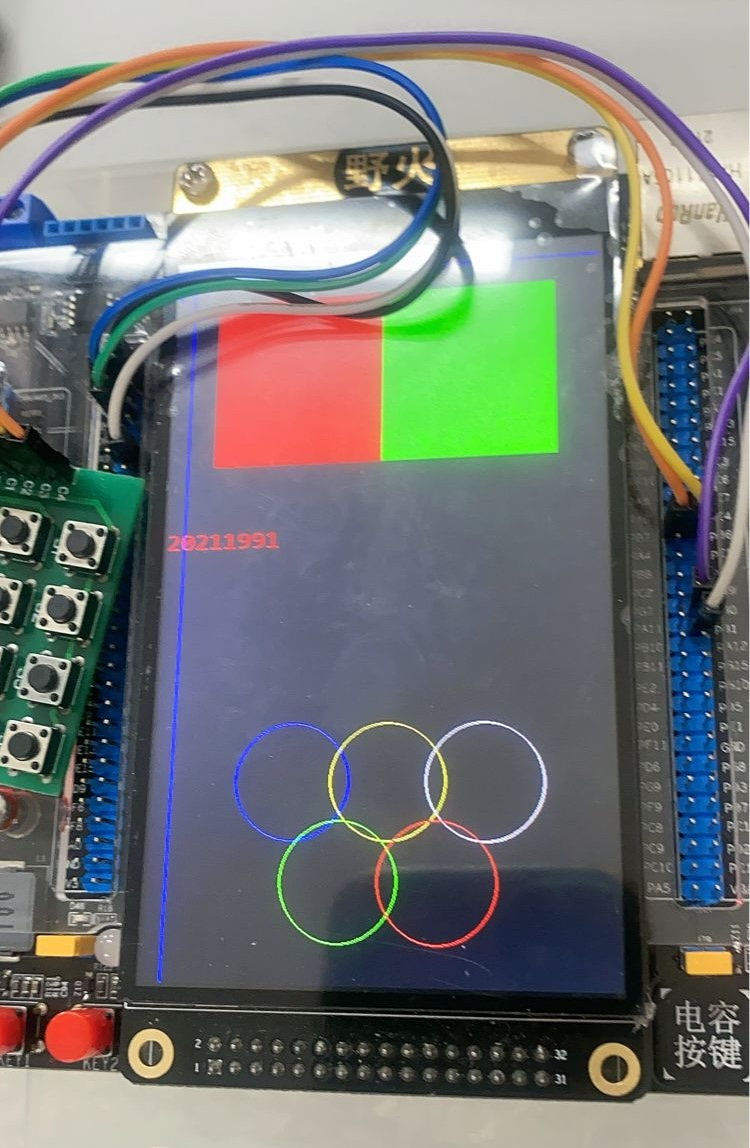
\includegraphics[width=0.6\linewidth]{lcd_result.jpg}
  \caption{LCD显示实验}      
\end{figure}

\subsubsection{在 LCD 上显示自己的一卡通图片}

按照\texttt{4.3寸LCD图片显示说明文档}中的说明,我们可以在LCD上显示图片。

下面是我的一卡通图片。

\begin{figure}[H]
  \centering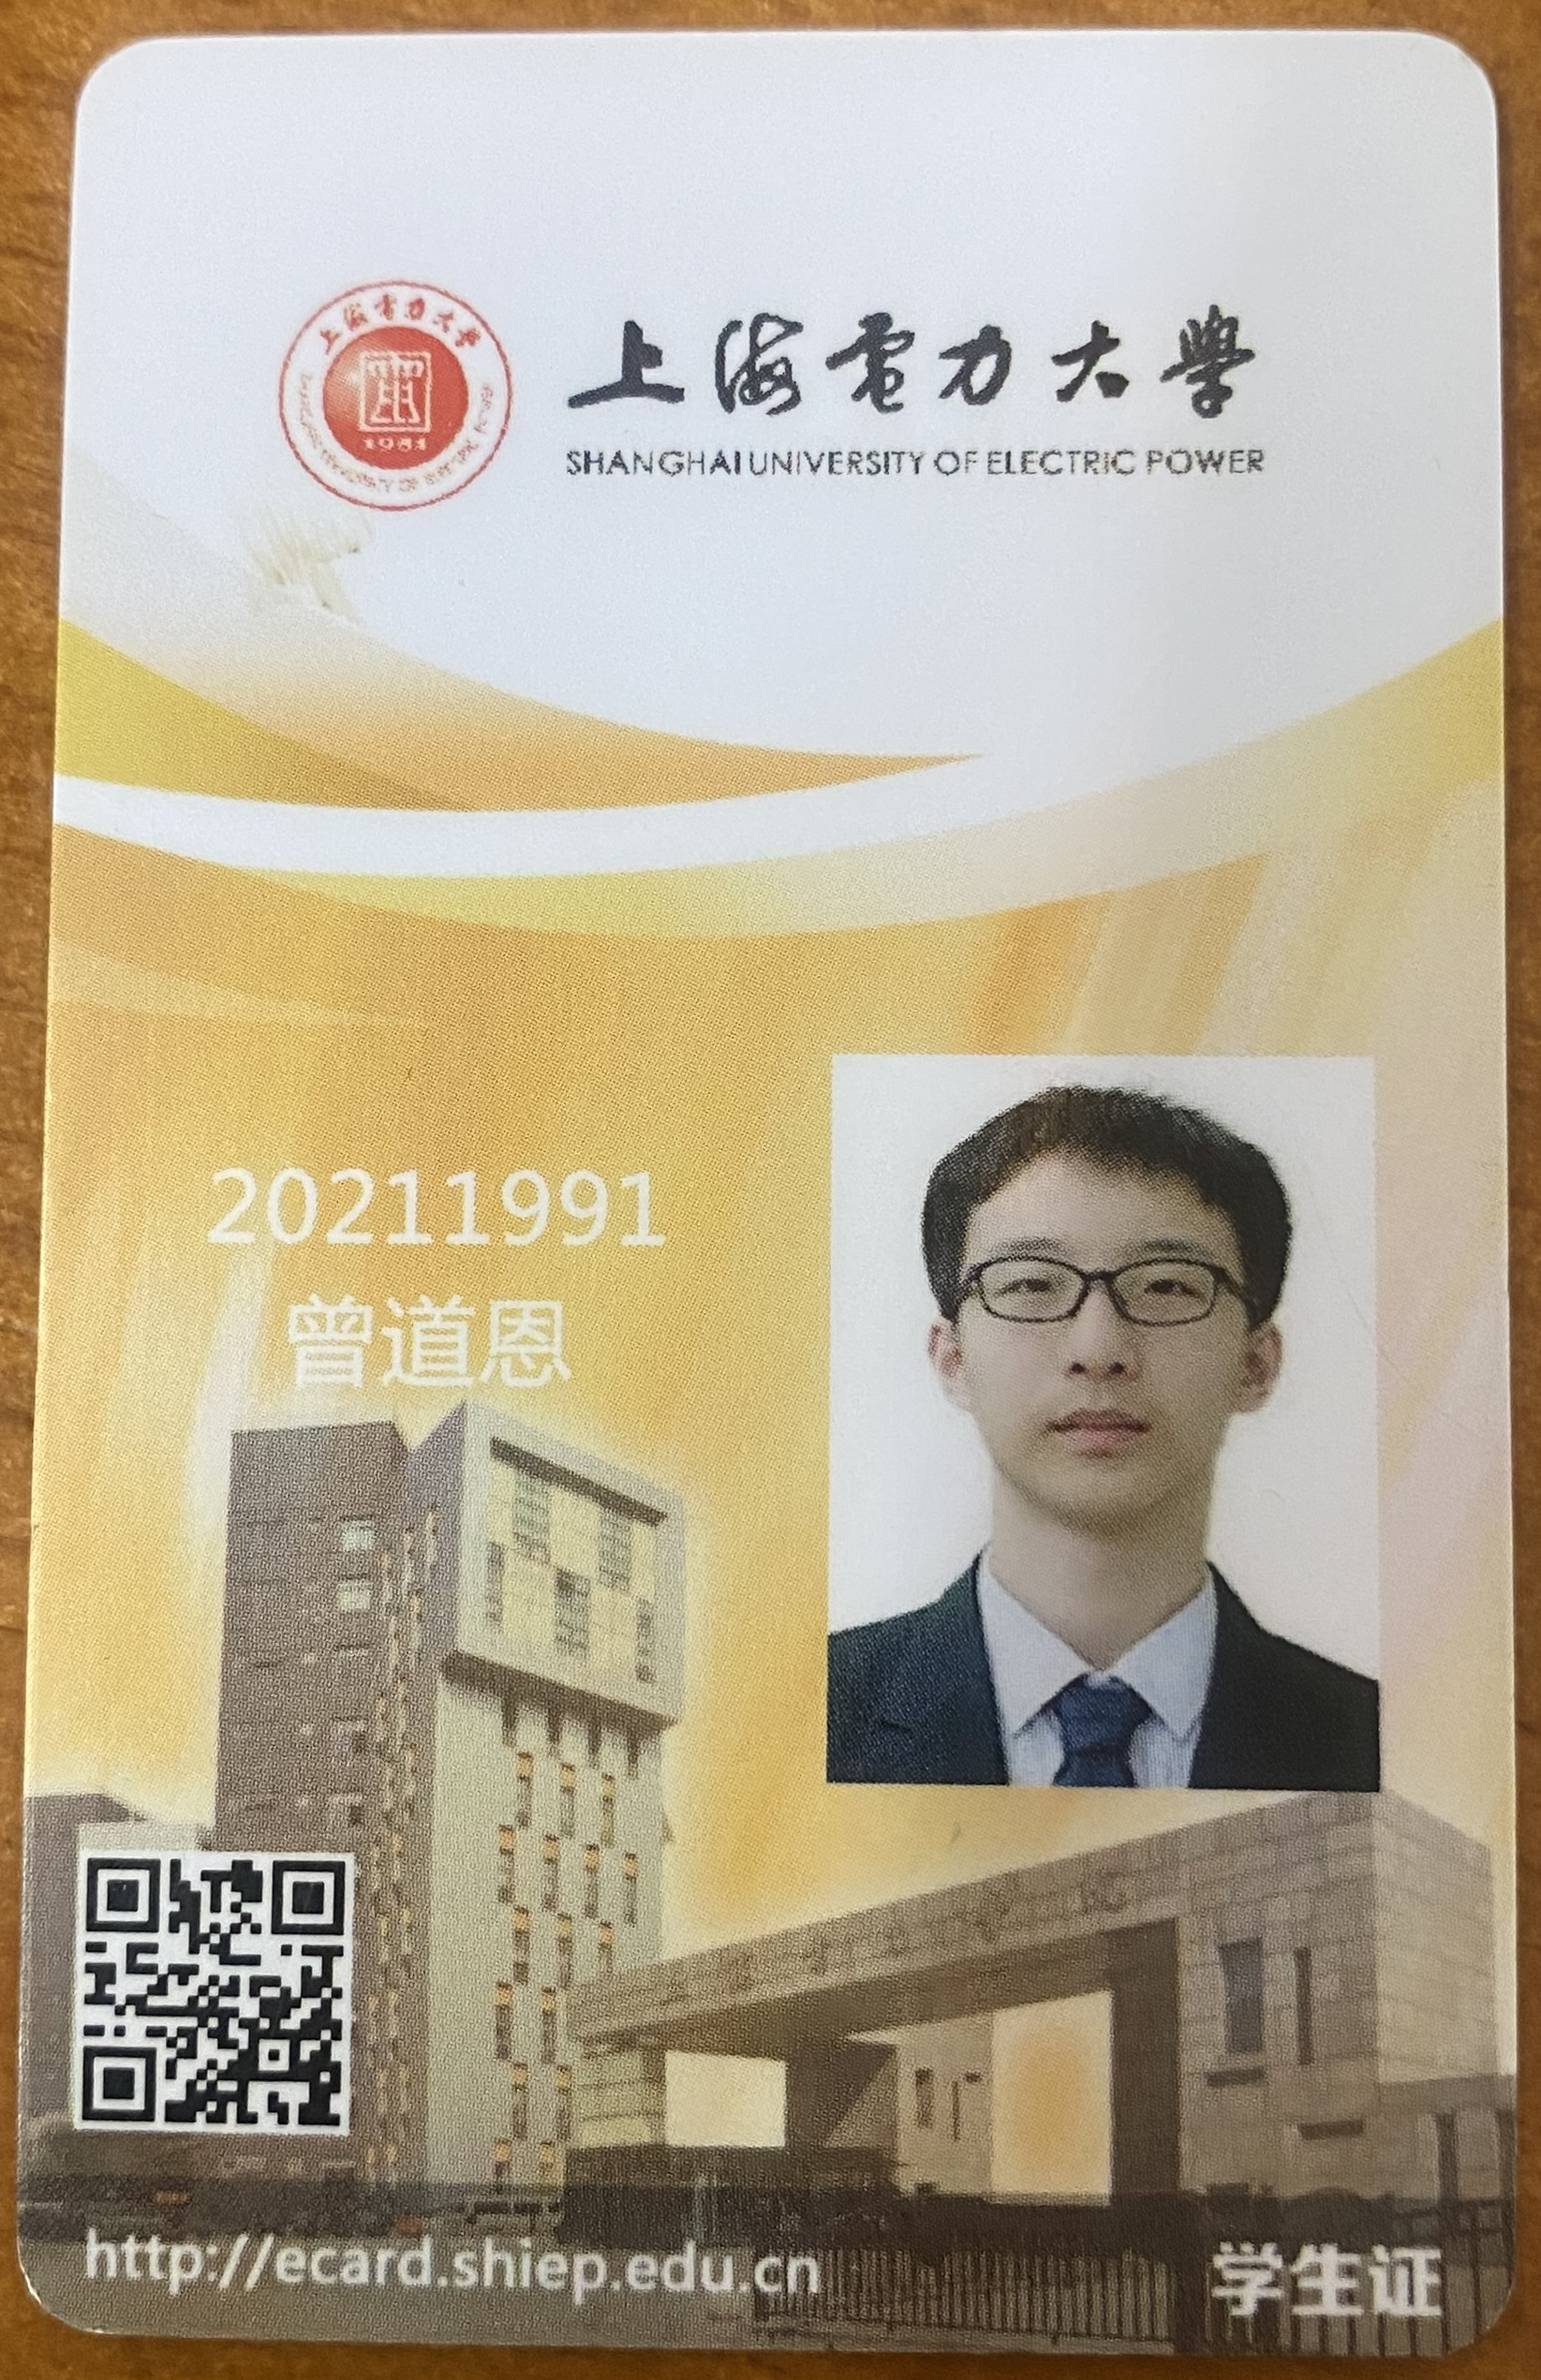
\includegraphics[width=0.6\linewidth]{2021xxxx.jpg}
  \caption{一卡通图片}      
\end{figure}

需要按照文档中的说明,将图片转换为\texttt{.h}文件,然后在\texttt{main.h}中引用。转换使用参数如图所示。

\begin{figure}[H]
  \centering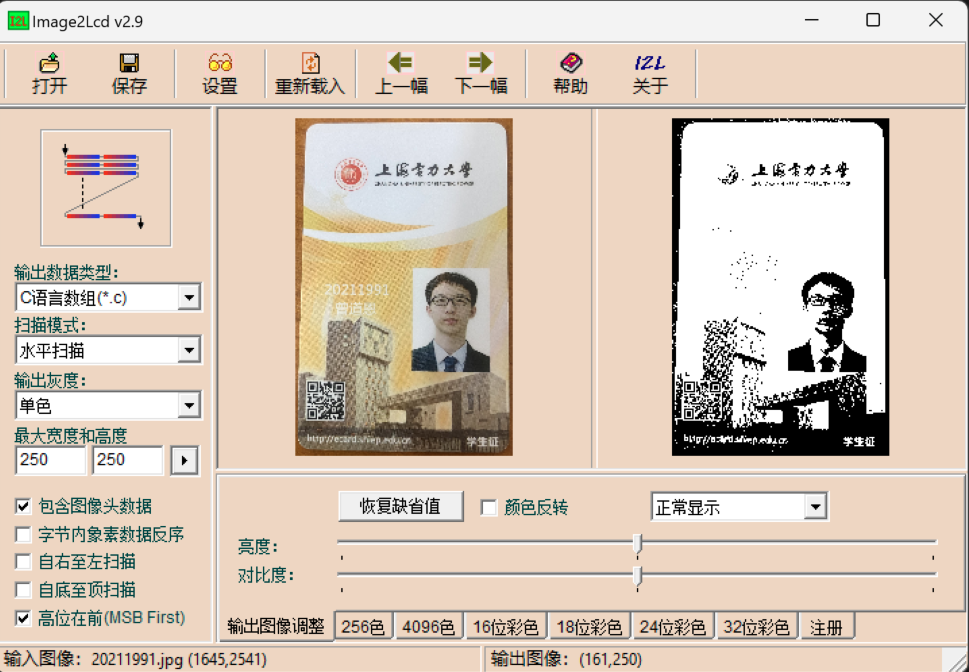
\includegraphics[width=0.6\linewidth]{lcd_img_convert.png}
  \caption{一卡通图片转换}
\end{figure}

最终的效果如下。

\begin{figure}[H]
  \centering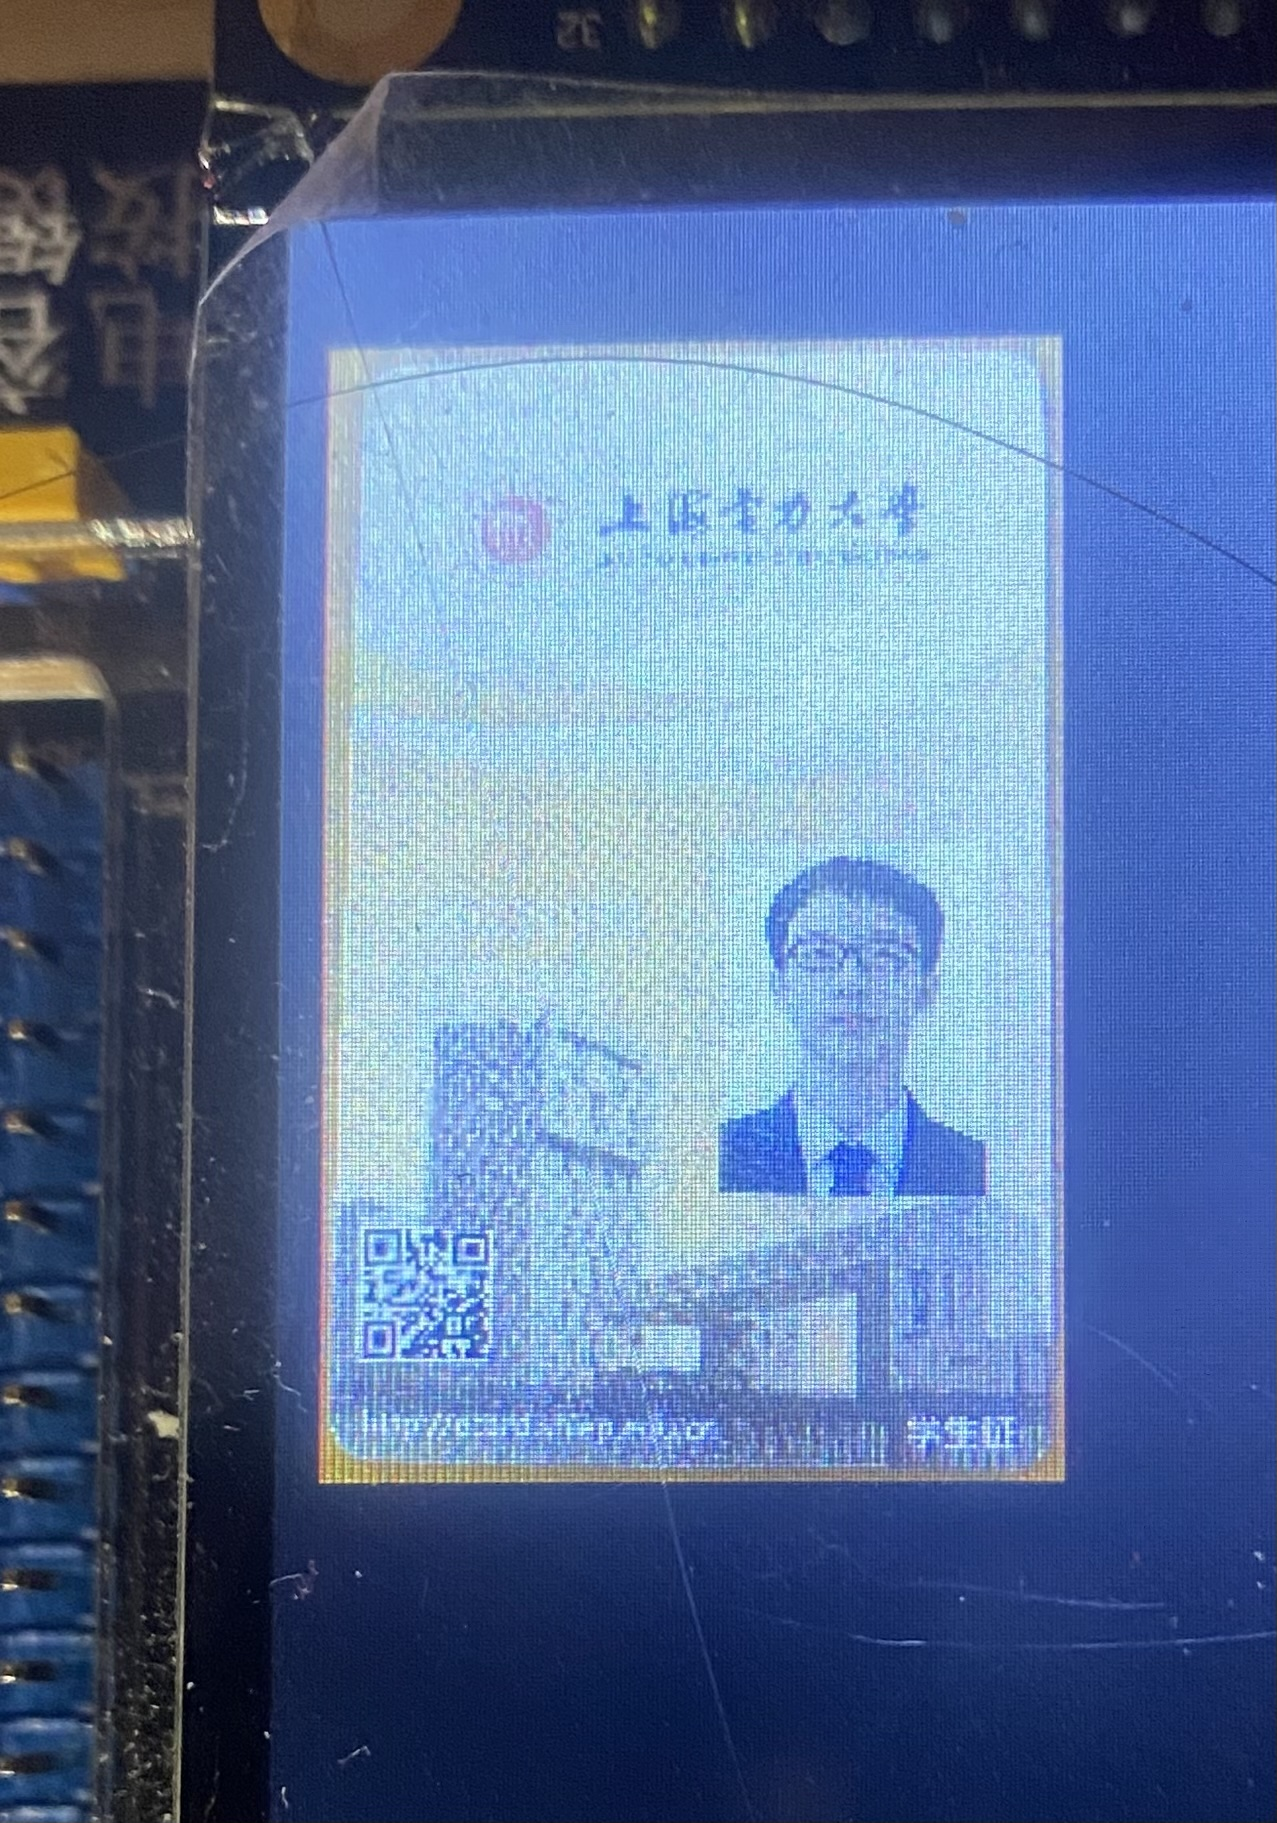
\includegraphics[width=0.6\linewidth]{lcd_img_result.jpg}
  \caption{一卡通图片显示效果}      
\end{figure}

\section{实验小结}

总之,本次实验让我们熟悉了液晶屏的基本操作和绘图功能。我们学到了如何初始化硬件、显示文本和绘制简单的图形。这对于进一步的液晶屏应用和项目开发非常有帮助。

\end{document}
